\documentclass[11pt]{article}

    \usepackage[breakable]{tcolorbox}
    \usepackage{parskip} % Stop auto-indenting (to mimic markdown behaviour)
    
    \usepackage{iftex}
    \ifPDFTeX
    	\usepackage[T1]{fontenc}
    	\usepackage{mathpazo}
    \else
    	\usepackage{fontspec}
    \fi

    \usepackage{graphicx} %package to manage images
    \graphicspath{ {./images/} }
    \usepackage{wrapfig}
    
    % Basic figure setup, for now with no caption control since it's done
    % automatically by Pandoc (which extracts ![](path) syntax from Markdown).
    \usepackage{graphicx}
    % Maintain compatibility with old templates. Remove in nbconvert 6.0
    \let\Oldincludegraphics\includegraphics
    % Ensure that by default, figures have no caption (until we provide a
    % proper Figure object with a Caption API and a way to capture that
    % in the conversion process - todo).
    \usepackage{caption}
    \DeclareCaptionFormat{nocaption}{}
    \captionsetup{format=nocaption,aboveskip=0pt,belowskip=0pt}

    \usepackage[Export]{adjustbox} % Used to constrain images to a maximum size
    \adjustboxset{max size={0.9\linewidth}{0.9\paperheight}}
    \usepackage{float}
    \floatplacement{figure}{H} % forces figures to be placed at the correct location
    \usepackage{xcolor} % Allow colors to be defined
    \usepackage{enumerate} % Needed for markdown enumerations to work
    \usepackage{geometry} % Used to adjust the document margins
    \usepackage{amsmath} % Equations
    \usepackage{amssymb} % Equations
    \usepackage{textcomp} % defines textquotesingle
    % Hack from http://tex.stackexchange.com/a/47451/13684:
    \AtBeginDocument{%
        \def\PYZsq{\textquotesingle}% Upright quotes in Pygmentized code
    }
    \usepackage{upquote} % Upright quotes for verbatim code
    \usepackage{eurosym} % defines \euro
    \usepackage[mathletters]{ucs} % Extended unicode (utf-8) support
    \usepackage{fancyvrb} % verbatim replacement that allows latex
    \usepackage{grffile} % extends the file name processing of package graphics 
                         % to support a larger range
    \makeatletter % fix for grffile with XeLaTeX
    \def\Gread@@xetex#1{%
      \IfFileExists{"\Gin@base".bb}%
      {\Gread@eps{\Gin@base.bb}}%
      {\Gread@@xetex@aux#1}%
    }
    \makeatother

    % The hyperref package gives us a pdf with properly built
    % internal navigation ('pdf bookmarks' for the table of contents,
    % internal cross-reference links, web links for URLs, etc.)
    \usepackage{hyperref}
    % The default LaTeX title has an obnoxious amount of whitespace. By default,
    % titling removes some of it. It also provides customization options.
    \usepackage{titling}
    \usepackage{longtable} % longtable support required by pandoc >1.10
    \usepackage{booktabs}  % table support for pandoc > 1.12.2
    \usepackage[inline]{enumitem} % IRkernel/repr support (it uses the enumerate* environment)
    \usepackage[normalem]{ulem} % ulem is needed to support strikethroughs (\sout)
                                % normalem makes italics be italics, not underlines
    \usepackage{mathrsfs}
    

    
    % Colors for the hyperref package
    \definecolor{urlcolor}{rgb}{0,.145,.698}
    \definecolor{linkcolor}{rgb}{.71,0.21,0.01}
    \definecolor{citecolor}{rgb}{.12,.54,.11}

    % ANSI colors
    \definecolor{ansi-black}{HTML}{3E424D}
    \definecolor{ansi-black-intense}{HTML}{282C36}
    \definecolor{ansi-red}{HTML}{E75C58}
    \definecolor{ansi-red-intense}{HTML}{B22B31}
    \definecolor{ansi-green}{HTML}{00A250}
    \definecolor{ansi-green-intense}{HTML}{007427}
    \definecolor{ansi-yellow}{HTML}{DDB62B}
    \definecolor{ansi-yellow-intense}{HTML}{B27D12}
    \definecolor{ansi-blue}{HTML}{208FFB}
    \definecolor{ansi-blue-intense}{HTML}{0065CA}
    \definecolor{ansi-magenta}{HTML}{D160C4}
    \definecolor{ansi-magenta-intense}{HTML}{A03196}
    \definecolor{ansi-cyan}{HTML}{60C6C8}
    \definecolor{ansi-cyan-intense}{HTML}{258F8F}
    \definecolor{ansi-white}{HTML}{C5C1B4}
    \definecolor{ansi-white-intense}{HTML}{A1A6B2}
    \definecolor{ansi-default-inverse-fg}{HTML}{FFFFFF}
    \definecolor{ansi-default-inverse-bg}{HTML}{000000}

    % commands and environments needed by pandoc snippets
    % extracted from the output of `pandoc -s`
    \providecommand{\tightlist}{%
      \setlength{\itemsep}{0pt}\setlength{\parskip}{0pt}}
    \DefineVerbatimEnvironment{Highlighting}{Verbatim}{commandchars=\\\{\}}
    % Add ',fontsize=\small' for more characters per line
    \newenvironment{Shaded}{}{}
    \newcommand{\KeywordTok}[1]{\textcolor[rgb]{0.00,0.44,0.13}{\textbf{{#1}}}}
    \newcommand{\DataTypeTok}[1]{\textcolor[rgb]{0.56,0.13,0.00}{{#1}}}
    \newcommand{\DecValTok}[1]{\textcolor[rgb]{0.25,0.63,0.44}{{#1}}}
    \newcommand{\BaseNTok}[1]{\textcolor[rgb]{0.25,0.63,0.44}{{#1}}}
    \newcommand{\FloatTok}[1]{\textcolor[rgb]{0.25,0.63,0.44}{{#1}}}
    \newcommand{\CharTok}[1]{\textcolor[rgb]{0.25,0.44,0.63}{{#1}}}
    \newcommand{\StringTok}[1]{\textcolor[rgb]{0.25,0.44,0.63}{{#1}}}
    \newcommand{\CommentTok}[1]{\textcolor[rgb]{0.38,0.63,0.69}{\textit{{#1}}}}
    \newcommand{\OtherTok}[1]{\textcolor[rgb]{0.00,0.44,0.13}{{#1}}}
    \newcommand{\AlertTok}[1]{\textcolor[rgb]{1.00,0.00,0.00}{\textbf{{#1}}}}
    \newcommand{\FunctionTok}[1]{\textcolor[rgb]{0.02,0.16,0.49}{{#1}}}
    \newcommand{\RegionMarkerTok}[1]{{#1}}
    \newcommand{\ErrorTok}[1]{\textcolor[rgb]{1.00,0.00,0.00}{\textbf{{#1}}}}
    \newcommand{\NormalTok}[1]{{#1}}
    
    % Additional commands for more recent versions of Pandoc
    \newcommand{\ConstantTok}[1]{\textcolor[rgb]{0.53,0.00,0.00}{{#1}}}
    \newcommand{\SpecialCharTok}[1]{\textcolor[rgb]{0.25,0.44,0.63}{{#1}}}
    \newcommand{\VerbatimStringTok}[1]{\textcolor[rgb]{0.25,0.44,0.63}{{#1}}}
    \newcommand{\SpecialStringTok}[1]{\textcolor[rgb]{0.73,0.40,0.53}{{#1}}}
    \newcommand{\ImportTok}[1]{{#1}}
    \newcommand{\DocumentationTok}[1]{\textcolor[rgb]{0.73,0.13,0.13}{\textit{{#1}}}}
    \newcommand{\AnnotationTok}[1]{\textcolor[rgb]{0.38,0.63,0.69}{\textbf{\textit{{#1}}}}}
    \newcommand{\CommentVarTok}[1]{\textcolor[rgb]{0.38,0.63,0.69}{\textbf{\textit{{#1}}}}}
    \newcommand{\VariableTok}[1]{\textcolor[rgb]{0.10,0.09,0.49}{{#1}}}
    \newcommand{\ControlFlowTok}[1]{\textcolor[rgb]{0.00,0.44,0.13}{\textbf{{#1}}}}
    \newcommand{\OperatorTok}[1]{\textcolor[rgb]{0.40,0.40,0.40}{{#1}}}
    \newcommand{\BuiltInTok}[1]{{#1}}
    \newcommand{\ExtensionTok}[1]{{#1}}
    \newcommand{\PreprocessorTok}[1]{\textcolor[rgb]{0.74,0.48,0.00}{{#1}}}
    \newcommand{\AttributeTok}[1]{\textcolor[rgb]{0.49,0.56,0.16}{{#1}}}
    \newcommand{\InformationTok}[1]{\textcolor[rgb]{0.38,0.63,0.69}{\textbf{\textit{{#1}}}}}
    \newcommand{\WarningTok}[1]{\textcolor[rgb]{0.38,0.63,0.69}{\textbf{\textit{{#1}}}}}
    
    
    % Define a nice break command that doesn't care if a line doesn't already
    % exist.
    \def\br{\hspace*{\fill} \\* }
    % Math Jax compatibility definitions
    \def\gt{>}
    \def\lt{<}
    \let\Oldtex\TeX
    \let\Oldlatex\LaTeX
    \renewcommand{\TeX}{\textrm{\Oldtex}}
    \renewcommand{\LaTeX}{\textrm{\Oldlatex}}
    % Document parameters
    % Document title
    \title{2-factor-Hull-White\_model\_calibration}
    
    
    
    
    
% Pygments definitions
\makeatletter
\def\PY@reset{\let\PY@it=\relax \let\PY@bf=\relax%
    \let\PY@ul=\relax \let\PY@tc=\relax%
    \let\PY@bc=\relax \let\PY@ff=\relax}
\def\PY@tok#1{\csname PY@tok@#1\endcsname}
\def\PY@toks#1+{\ifx\relax#1\empty\else%
    \PY@tok{#1}\expandafter\PY@toks\fi}
\def\PY@do#1{\PY@bc{\PY@tc{\PY@ul{%
    \PY@it{\PY@bf{\PY@ff{#1}}}}}}}
\def\PY#1#2{\PY@reset\PY@toks#1+\relax+\PY@do{#2}}

\expandafter\def\csname PY@tok@w\endcsname{\def\PY@tc##1{\textcolor[rgb]{0.73,0.73,0.73}{##1}}}
\expandafter\def\csname PY@tok@c\endcsname{\let\PY@it=\textit\def\PY@tc##1{\textcolor[rgb]{0.25,0.50,0.50}{##1}}}
\expandafter\def\csname PY@tok@cp\endcsname{\def\PY@tc##1{\textcolor[rgb]{0.74,0.48,0.00}{##1}}}
\expandafter\def\csname PY@tok@k\endcsname{\let\PY@bf=\textbf\def\PY@tc##1{\textcolor[rgb]{0.00,0.50,0.00}{##1}}}
\expandafter\def\csname PY@tok@kp\endcsname{\def\PY@tc##1{\textcolor[rgb]{0.00,0.50,0.00}{##1}}}
\expandafter\def\csname PY@tok@kt\endcsname{\def\PY@tc##1{\textcolor[rgb]{0.69,0.00,0.25}{##1}}}
\expandafter\def\csname PY@tok@o\endcsname{\def\PY@tc##1{\textcolor[rgb]{0.40,0.40,0.40}{##1}}}
\expandafter\def\csname PY@tok@ow\endcsname{\let\PY@bf=\textbf\def\PY@tc##1{\textcolor[rgb]{0.67,0.13,1.00}{##1}}}
\expandafter\def\csname PY@tok@nb\endcsname{\def\PY@tc##1{\textcolor[rgb]{0.00,0.50,0.00}{##1}}}
\expandafter\def\csname PY@tok@nf\endcsname{\def\PY@tc##1{\textcolor[rgb]{0.00,0.00,1.00}{##1}}}
\expandafter\def\csname PY@tok@nc\endcsname{\let\PY@bf=\textbf\def\PY@tc##1{\textcolor[rgb]{0.00,0.00,1.00}{##1}}}
\expandafter\def\csname PY@tok@nn\endcsname{\let\PY@bf=\textbf\def\PY@tc##1{\textcolor[rgb]{0.00,0.00,1.00}{##1}}}
\expandafter\def\csname PY@tok@ne\endcsname{\let\PY@bf=\textbf\def\PY@tc##1{\textcolor[rgb]{0.82,0.25,0.23}{##1}}}
\expandafter\def\csname PY@tok@nv\endcsname{\def\PY@tc##1{\textcolor[rgb]{0.10,0.09,0.49}{##1}}}
\expandafter\def\csname PY@tok@no\endcsname{\def\PY@tc##1{\textcolor[rgb]{0.53,0.00,0.00}{##1}}}
\expandafter\def\csname PY@tok@nl\endcsname{\def\PY@tc##1{\textcolor[rgb]{0.63,0.63,0.00}{##1}}}
\expandafter\def\csname PY@tok@ni\endcsname{\let\PY@bf=\textbf\def\PY@tc##1{\textcolor[rgb]{0.60,0.60,0.60}{##1}}}
\expandafter\def\csname PY@tok@na\endcsname{\def\PY@tc##1{\textcolor[rgb]{0.49,0.56,0.16}{##1}}}
\expandafter\def\csname PY@tok@nt\endcsname{\let\PY@bf=\textbf\def\PY@tc##1{\textcolor[rgb]{0.00,0.50,0.00}{##1}}}
\expandafter\def\csname PY@tok@nd\endcsname{\def\PY@tc##1{\textcolor[rgb]{0.67,0.13,1.00}{##1}}}
\expandafter\def\csname PY@tok@s\endcsname{\def\PY@tc##1{\textcolor[rgb]{0.73,0.13,0.13}{##1}}}
\expandafter\def\csname PY@tok@sd\endcsname{\let\PY@it=\textit\def\PY@tc##1{\textcolor[rgb]{0.73,0.13,0.13}{##1}}}
\expandafter\def\csname PY@tok@si\endcsname{\let\PY@bf=\textbf\def\PY@tc##1{\textcolor[rgb]{0.73,0.40,0.53}{##1}}}
\expandafter\def\csname PY@tok@se\endcsname{\let\PY@bf=\textbf\def\PY@tc##1{\textcolor[rgb]{0.73,0.40,0.13}{##1}}}
\expandafter\def\csname PY@tok@sr\endcsname{\def\PY@tc##1{\textcolor[rgb]{0.73,0.40,0.53}{##1}}}
\expandafter\def\csname PY@tok@ss\endcsname{\def\PY@tc##1{\textcolor[rgb]{0.10,0.09,0.49}{##1}}}
\expandafter\def\csname PY@tok@sx\endcsname{\def\PY@tc##1{\textcolor[rgb]{0.00,0.50,0.00}{##1}}}
\expandafter\def\csname PY@tok@m\endcsname{\def\PY@tc##1{\textcolor[rgb]{0.40,0.40,0.40}{##1}}}
\expandafter\def\csname PY@tok@gh\endcsname{\let\PY@bf=\textbf\def\PY@tc##1{\textcolor[rgb]{0.00,0.00,0.50}{##1}}}
\expandafter\def\csname PY@tok@gu\endcsname{\let\PY@bf=\textbf\def\PY@tc##1{\textcolor[rgb]{0.50,0.00,0.50}{##1}}}
\expandafter\def\csname PY@tok@gd\endcsname{\def\PY@tc##1{\textcolor[rgb]{0.63,0.00,0.00}{##1}}}
\expandafter\def\csname PY@tok@gi\endcsname{\def\PY@tc##1{\textcolor[rgb]{0.00,0.63,0.00}{##1}}}
\expandafter\def\csname PY@tok@gr\endcsname{\def\PY@tc##1{\textcolor[rgb]{1.00,0.00,0.00}{##1}}}
\expandafter\def\csname PY@tok@ge\endcsname{\let\PY@it=\textit}
\expandafter\def\csname PY@tok@gs\endcsname{\let\PY@bf=\textbf}
\expandafter\def\csname PY@tok@gp\endcsname{\let\PY@bf=\textbf\def\PY@tc##1{\textcolor[rgb]{0.00,0.00,0.50}{##1}}}
\expandafter\def\csname PY@tok@go\endcsname{\def\PY@tc##1{\textcolor[rgb]{0.53,0.53,0.53}{##1}}}
\expandafter\def\csname PY@tok@gt\endcsname{\def\PY@tc##1{\textcolor[rgb]{0.00,0.27,0.87}{##1}}}
\expandafter\def\csname PY@tok@err\endcsname{\def\PY@bc##1{\setlength{\fboxsep}{0pt}\fcolorbox[rgb]{1.00,0.00,0.00}{1,1,1}{\strut ##1}}}
\expandafter\def\csname PY@tok@kc\endcsname{\let\PY@bf=\textbf\def\PY@tc##1{\textcolor[rgb]{0.00,0.50,0.00}{##1}}}
\expandafter\def\csname PY@tok@kd\endcsname{\let\PY@bf=\textbf\def\PY@tc##1{\textcolor[rgb]{0.00,0.50,0.00}{##1}}}
\expandafter\def\csname PY@tok@kn\endcsname{\let\PY@bf=\textbf\def\PY@tc##1{\textcolor[rgb]{0.00,0.50,0.00}{##1}}}
\expandafter\def\csname PY@tok@kr\endcsname{\let\PY@bf=\textbf\def\PY@tc##1{\textcolor[rgb]{0.00,0.50,0.00}{##1}}}
\expandafter\def\csname PY@tok@bp\endcsname{\def\PY@tc##1{\textcolor[rgb]{0.00,0.50,0.00}{##1}}}
\expandafter\def\csname PY@tok@fm\endcsname{\def\PY@tc##1{\textcolor[rgb]{0.00,0.00,1.00}{##1}}}
\expandafter\def\csname PY@tok@vc\endcsname{\def\PY@tc##1{\textcolor[rgb]{0.10,0.09,0.49}{##1}}}
\expandafter\def\csname PY@tok@vg\endcsname{\def\PY@tc##1{\textcolor[rgb]{0.10,0.09,0.49}{##1}}}
\expandafter\def\csname PY@tok@vi\endcsname{\def\PY@tc##1{\textcolor[rgb]{0.10,0.09,0.49}{##1}}}
\expandafter\def\csname PY@tok@vm\endcsname{\def\PY@tc##1{\textcolor[rgb]{0.10,0.09,0.49}{##1}}}
\expandafter\def\csname PY@tok@sa\endcsname{\def\PY@tc##1{\textcolor[rgb]{0.73,0.13,0.13}{##1}}}
\expandafter\def\csname PY@tok@sb\endcsname{\def\PY@tc##1{\textcolor[rgb]{0.73,0.13,0.13}{##1}}}
\expandafter\def\csname PY@tok@sc\endcsname{\def\PY@tc##1{\textcolor[rgb]{0.73,0.13,0.13}{##1}}}
\expandafter\def\csname PY@tok@dl\endcsname{\def\PY@tc##1{\textcolor[rgb]{0.73,0.13,0.13}{##1}}}
\expandafter\def\csname PY@tok@s2\endcsname{\def\PY@tc##1{\textcolor[rgb]{0.73,0.13,0.13}{##1}}}
\expandafter\def\csname PY@tok@sh\endcsname{\def\PY@tc##1{\textcolor[rgb]{0.73,0.13,0.13}{##1}}}
\expandafter\def\csname PY@tok@s1\endcsname{\def\PY@tc##1{\textcolor[rgb]{0.73,0.13,0.13}{##1}}}
\expandafter\def\csname PY@tok@mb\endcsname{\def\PY@tc##1{\textcolor[rgb]{0.40,0.40,0.40}{##1}}}
\expandafter\def\csname PY@tok@mf\endcsname{\def\PY@tc##1{\textcolor[rgb]{0.40,0.40,0.40}{##1}}}
\expandafter\def\csname PY@tok@mh\endcsname{\def\PY@tc##1{\textcolor[rgb]{0.40,0.40,0.40}{##1}}}
\expandafter\def\csname PY@tok@mi\endcsname{\def\PY@tc##1{\textcolor[rgb]{0.40,0.40,0.40}{##1}}}
\expandafter\def\csname PY@tok@il\endcsname{\def\PY@tc##1{\textcolor[rgb]{0.40,0.40,0.40}{##1}}}
\expandafter\def\csname PY@tok@mo\endcsname{\def\PY@tc##1{\textcolor[rgb]{0.40,0.40,0.40}{##1}}}
\expandafter\def\csname PY@tok@ch\endcsname{\let\PY@it=\textit\def\PY@tc##1{\textcolor[rgb]{0.25,0.50,0.50}{##1}}}
\expandafter\def\csname PY@tok@cm\endcsname{\let\PY@it=\textit\def\PY@tc##1{\textcolor[rgb]{0.25,0.50,0.50}{##1}}}
\expandafter\def\csname PY@tok@cpf\endcsname{\let\PY@it=\textit\def\PY@tc##1{\textcolor[rgb]{0.25,0.50,0.50}{##1}}}
\expandafter\def\csname PY@tok@c1\endcsname{\let\PY@it=\textit\def\PY@tc##1{\textcolor[rgb]{0.25,0.50,0.50}{##1}}}
\expandafter\def\csname PY@tok@cs\endcsname{\let\PY@it=\textit\def\PY@tc##1{\textcolor[rgb]{0.25,0.50,0.50}{##1}}}

\def\PYZbs{\char`\\}
\def\PYZus{\char`\_}
\def\PYZob{\char`\{}
\def\PYZcb{\char`\}}
\def\PYZca{\char`\^}
\def\PYZam{\char`\&}
\def\PYZlt{\char`\<}
\def\PYZgt{\char`\>}
\def\PYZsh{\char`\#}
\def\PYZpc{\char`\%}
\def\PYZdl{\char`\$}
\def\PYZhy{\char`\-}
\def\PYZsq{\char`\'}
\def\PYZdq{\char`\"}
\def\PYZti{\char`\~}
% for compatibility with earlier versions
\def\PYZat{@}
\def\PYZlb{[}
\def\PYZrb{]}
\makeatother


    % For linebreaks inside Verbatim environment from package fancyvrb. 
    \makeatletter
        \newbox\Wrappedcontinuationbox 
        \newbox\Wrappedvisiblespacebox 
        \newcommand*\Wrappedvisiblespace {\textcolor{red}{\textvisiblespace}} 
        \newcommand*\Wrappedcontinuationsymbol {\textcolor{red}{\llap{\tiny$\m@th\hookrightarrow$}}} 
        \newcommand*\Wrappedcontinuationindent {3ex } 
        \newcommand*\Wrappedafterbreak {\kern\Wrappedcontinuationindent\copy\Wrappedcontinuationbox} 
        % Take advantage of the already applied Pygments mark-up to insert 
        % potential linebreaks for TeX processing. 
        %        {, <, #, %, $, ' and ": go to next line. 
        %        _, }, ^, &, >, - and ~: stay at end of broken line. 
        % Use of \textquotesingle for straight quote. 
        \newcommand*\Wrappedbreaksatspecials {% 
            \def\PYGZus{\discretionary{\char`\_}{\Wrappedafterbreak}{\char`\_}}% 
            \def\PYGZob{\discretionary{}{\Wrappedafterbreak\char`\{}{\char`\{}}% 
            \def\PYGZcb{\discretionary{\char`\}}{\Wrappedafterbreak}{\char`\}}}% 
            \def\PYGZca{\discretionary{\char`\^}{\Wrappedafterbreak}{\char`\^}}% 
            \def\PYGZam{\discretionary{\char`\&}{\Wrappedafterbreak}{\char`\&}}% 
            \def\PYGZlt{\discretionary{}{\Wrappedafterbreak\char`\<}{\char`\<}}% 
            \def\PYGZgt{\discretionary{\char`\>}{\Wrappedafterbreak}{\char`\>}}% 
            \def\PYGZsh{\discretionary{}{\Wrappedafterbreak\char`\#}{\char`\#}}% 
            \def\PYGZpc{\discretionary{}{\Wrappedafterbreak\char`\%}{\char`\%}}% 
            \def\PYGZdl{\discretionary{}{\Wrappedafterbreak\char`\$}{\char`\$}}% 
            \def\PYGZhy{\discretionary{\char`\-}{\Wrappedafterbreak}{\char`\-}}% 
            \def\PYGZsq{\discretionary{}{\Wrappedafterbreak\textquotesingle}{\textquotesingle}}% 
            \def\PYGZdq{\discretionary{}{\Wrappedafterbreak\char`\"}{\char`\"}}% 
            \def\PYGZti{\discretionary{\char`\~}{\Wrappedafterbreak}{\char`\~}}% 
        } 
        % Some characters . , ; ? ! / are not pygmentized. 
        % This macro makes them "active" and they will insert potential linebreaks 
        \newcommand*\Wrappedbreaksatpunct {% 
            \lccode`\~`\.\lowercase{\def~}{\discretionary{\hbox{\char`\.}}{\Wrappedafterbreak}{\hbox{\char`\.}}}% 
            \lccode`\~`\,\lowercase{\def~}{\discretionary{\hbox{\char`\,}}{\Wrappedafterbreak}{\hbox{\char`\,}}}% 
            \lccode`\~`\;\lowercase{\def~}{\discretionary{\hbox{\char`\;}}{\Wrappedafterbreak}{\hbox{\char`\;}}}% 
            \lccode`\~`\:\lowercase{\def~}{\discretionary{\hbox{\char`\:}}{\Wrappedafterbreak}{\hbox{\char`\:}}}% 
            \lccode`\~`\?\lowercase{\def~}{\discretionary{\hbox{\char`\?}}{\Wrappedafterbreak}{\hbox{\char`\?}}}% 
            \lccode`\~`\!\lowercase{\def~}{\discretionary{\hbox{\char`\!}}{\Wrappedafterbreak}{\hbox{\char`\!}}}% 
            \lccode`\~`\/\lowercase{\def~}{\discretionary{\hbox{\char`\/}}{\Wrappedafterbreak}{\hbox{\char`\/}}}% 
            \catcode`\.\active
            \catcode`\,\active 
            \catcode`\;\active
            \catcode`\:\active
            \catcode`\?\active
            \catcode`\!\active
            \catcode`\/\active 
            \lccode`\~`\~ 	
        }
    \makeatother

    \let\OriginalVerbatim=\Verbatim
    \makeatletter
    \renewcommand{\Verbatim}[1][1]{%
        %\parskip\z@skip
        \sbox\Wrappedcontinuationbox {\Wrappedcontinuationsymbol}%
        \sbox\Wrappedvisiblespacebox {\FV@SetupFont\Wrappedvisiblespace}%
        \def\FancyVerbFormatLine ##1{\hsize\linewidth
            \vtop{\raggedright\hyphenpenalty\z@\exhyphenpenalty\z@
                \doublehyphendemerits\z@\finalhyphendemerits\z@
                \strut ##1\strut}%
        }%
        % If the linebreak is at a space, the latter will be displayed as visible
        % space at end of first line, and a continuation symbol starts next line.
        % Stretch/shrink are however usually zero for typewriter font.
        \def\FV@Space {%
            \nobreak\hskip\z@ plus\fontdimen3\font minus\fontdimen4\font
            \discretionary{\copy\Wrappedvisiblespacebox}{\Wrappedafterbreak}
            {\kern\fontdimen2\font}%
        }%
        
        % Allow breaks at special characters using \PYG... macros.
        \Wrappedbreaksatspecials
        % Breaks at punctuation characters . , ; ? ! and / need catcode=\active 	
        \OriginalVerbatim[#1,codes*=\Wrappedbreaksatpunct]%
    }
    \makeatother

    % Exact colors from NB
    \definecolor{incolor}{HTML}{303F9F}
    \definecolor{outcolor}{HTML}{D84315}
    \definecolor{cellborder}{HTML}{CFCFCF}
    \definecolor{cellbackground}{HTML}{F7F7F7}
    
    % prompt
    \makeatletter
    \newcommand{\boxspacing}{\kern\kvtcb@left@rule\kern\kvtcb@boxsep}
    \makeatother
    \newcommand{\prompt}[4]{
        \ttfamily\llap{{\color{#2}[#3]:\hspace{3pt}#4}}\vspace{-\baselineskip}
    }
    

    
    % Prevent overflowing lines due to hard-to-break entities
    \sloppy 
    % Setup hyperref package
    \hypersetup{
      breaklinks=true,  % so long urls are correctly broken across lines
      colorlinks=true,
      urlcolor=urlcolor,
      linkcolor=linkcolor,
      citecolor=citecolor,
      }
    % Slightly bigger margins than the latex defaults
    
    \geometry{verbose,tmargin=1in,bmargin=1in,lmargin=1in,rmargin=1in}
\begin{document}

\nocite{*} % this command forces all references in template.bib to be printed in the bibliography

\title{Price a European Up-and-out Call Option}

\author{
  Ng, Joe Hoong\\
  \texttt{ng\_joehoong@hotmail.com}
  \and
  Nguyen, Dang Duy Nghia \\
  \texttt{nghia002@e.ntu.edu.sg}
   \and
  Ansari, Zain Us Sami Ahmed \\
  \texttt{zainussami@gmail.com}  
   \and
   Thorne, Dylan \\
  \texttt{dylan.thorne@gmail.com}  
  }

\date{April. 8, 2020} % if this is omitted, the current date is used for the title page
\maketitle

\noindent
\textbf{Keywords:} Exotic Options, European up-and-out call option,  Black-Scholes-Merton model and Geometric Brownian Motion.



% the following creates an abstract -- it can be omitted
% an example of an environment: these have the form \begin{name} ... \end{name}
\begin{abstract}
This report presents the results of the simulation of a European up-and-out call option over twelve months.  The Black-Scholes-Merton model will be used to implement Monte Carlo estimations using Python code. The estimations will simulate paths for the underlying share and the counterparty's firm value using varying sample sizes, and determine estimates of both the default-free value of the option and the Credit Valuation Adjustment (CVA). Following from these it is simple to price the option incorporating counterparty risk, given by the default-free price less the CVA.
\end{abstract}

\section{Introduction
}
A European up-and-out call option is type of a Barrier Option, these options are consider path-dependant because barrier option's payoff is based on the underlying stock's price path.  The payoff of an up-and-out option at maturity $T$ is given by,

\[
Payoff_T= (S_T - K)^+ given, max_{t \in [0,T]} S_t < L
\]
Where, where $K$ is the strike of the option, $L$ is the barrier level, and $S_t$ is the share price at time $t$.  This is a type of call option whose payoff is reduced to 0 if the share price crosses the barrier level. \\

The seminal work of Merton \cite{Merton1} pioneered the formula for pricing barrier options.  This led pricing formulas under the geometric Brownian motion (GBM) framework for one-asset barrier options by Rich \cite{RD1} and multi-asset barrier options by Wong and Kwok \cite{WK1}. Although the return dynamics of underlying shares are not sufficiently well described by the GBM process proposed by Black and Scholes \cite{BS1}, we are going to assume both the stock and counterparty firm values follow GBM  with constant drift and volatilities and default only occurs at maturity.

Possible paths for the up-and-out barrier option payoff would look similar to the chart below, where two of the paths have crossed the barrier and resulted in zero payoff, but the other three have not crossed the barrier and behave like a vanilla option.

\begin{figure}
    \centering
    \caption{Simulated Payoffs for an Up-and-out Barrier Option}
    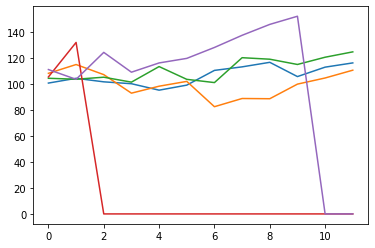
\includegraphics{images/barrier-example.png}
\end{figure}

We initialize most variables as given by the question. We assume the
counterparty firm's value is at 200, as this is above the counterparty's
debt due in one year. Also, we calculate the default-free value of our
option to be 6.60, so we select a firm value not too distant such that
the CVA value we calculate is not negligible. For example, if we chose
counterparty firm value as 1,000, the CVA would be 0.000.

    \begin{tcolorbox}[breakable, size=fbox, boxrule=1pt, pad at break*=1mm,colback=cellbackground, colframe=cellborder]
\prompt{In}{incolor}{2}{\boxspacing}
\begin{Verbatim}[commandchars=\\\{\}]
\PY{c+c1}{\PYZsh{}\PYZsh{}\PYZsh{} Initialize problem parameters}
\PY{n}{T} \PY{o}{=} \PY{l+m+mi}{1} \PY{c+c1}{\PYZsh{} option maturity}
\PY{n}{L} \PY{o}{=} \PY{l+m+mi}{150} \PY{c+c1}{\PYZsh{} up\PYZhy{}and\PYZhy{}out barrier}
\PY{n}{S0} \PY{o}{=} \PY{l+m+mi}{100} \PY{c+c1}{\PYZsh{} current share price}
\PY{n}{K} \PY{o}{=} \PY{l+m+mi}{100} \PY{c+c1}{\PYZsh{} strike price, at\PYZhy{}the\PYZhy{}money}
\PY{n}{risk\PYZus{}free} \PY{o}{=} \PY{o}{.}\PY{l+m+mi}{08} \PY{c+c1}{\PYZsh{} risk\PYZhy{}free rate}
\PY{n}{sigma} \PY{o}{=} \PY{o}{.}\PY{l+m+mi}{3} \PY{c+c1}{\PYZsh{} volatility}
\PY{n}{v\PYZus{}0} \PY{o}{=} \PY{l+m+mi}{200} \PY{c+c1}{\PYZsh{} counterparty firm current value (Our assumption) }
\PY{n}{sigma\PYZus{}firm} \PY{o}{=} \PY{o}{.}\PY{l+m+mi}{25} \PY{c+c1}{\PYZsh{} volatility for the counterparty\PYZsq{}s firm}
\PY{n}{debt} \PY{o}{=} \PY{l+m+mi}{175} \PY{c+c1}{\PYZsh{} counterparty\PYZsq{}s debt, due in one year }
\PY{n}{corr} \PY{o}{=} \PY{o}{.}\PY{l+m+mi}{2} \PY{c+c1}{\PYZsh{} correlation}
\PY{n}{recovery\PYZus{}rate} \PY{o}{=} \PY{l+m+mf}{0.25} \PY{c+c1}{\PYZsh{} recovery rate}
\PY{c+c1}{\PYZsh{}\PYZsh{}\PYZsh{}\PYZsh{}\PYZsh{}\PYZsh{}\PYZsh{}\PYZsh{}}
\PY{n}{corr\PYZus{}matrix} \PY{o}{=} \PY{n}{np}\PY{o}{.}\PY{n}{array}\PY{p}{(}\PY{p}{[}\PY{p}{[}\PY{l+m+mi}{1}\PY{p}{,} \PY{n}{corr}\PY{p}{]}\PY{p}{,} \PY{p}{[}\PY{n}{corr}\PY{p}{,} \PY{l+m+mi}{1}\PY{p}{]}\PY{p}{]}\PY{p}{)}
\PY{n}{sample\PYZus{}sizes} \PY{o}{=} \PY{n+nb}{range}\PY{p}{(}\PY{l+m+mi}{1000}\PY{p}{,} \PY{l+m+mi}{50001}\PY{p}{,} \PY{l+m+mi}{1000}\PY{p}{)}
\end{Verbatim}
\end{tcolorbox}

\section{Simulated Paths for the Underlying Share and Counterparty Firm
}

 In order to simulate paths for the underlying share and the firm,  we use a Cholesky decomposition to generate the correlated price paths.

    \begin{tcolorbox}[breakable, size=fbox, boxrule=1pt, pad at break*=1mm,colback=cellbackground, colframe=cellborder]
\prompt{In}{incolor}{3}{\boxspacing}
\begin{Verbatim}[commandchars=\\\{\}]
\PY{k}{def} \PY{n+nf}{share\PYZus{}path}\PY{p}{(}\PY{n}{S\PYZus{}0}\PY{p}{,} \PY{n}{risk\PYZus{}free\PYZus{}rate}\PY{p}{,} \PY{n}{sigma}\PY{p}{,} \PY{n}{Z}\PY{p}{,} \PY{n}{dT}\PY{p}{)}\PY{p}{:}
    \PY{k}{return} \PY{n}{S\PYZus{}0}\PY{o}{*}\PY{n}{np}\PY{o}{.}\PY{n}{exp}\PY{p}{(}\PY{n}{np}\PY{o}{.}\PY{n}{cumsum}\PY{p}{(}\PY{p}{(}\PY{n}{risk\PYZus{}free\PYZus{}rate}\PY{o}{\PYZhy{}}\PY{n}{sigma}\PY{o}{*}\PY{o}{*}\PY{l+m+mi}{2}\PY{o}{/}\PY{l+m+mi}{2}\PY{p}{)}\PY{o}{*}\PY{n}{dT} \PY{o}{+} \PY{n}{sigma}\PY{o}{*}\PY{n}{np}\PY{o}{.}\PY{n}{sqrt}\PY{p}{(}\PY{n}{dT}\PY{p}{)}\PY{o}{*}\PY{n}{Z}\PY{p}{,}\PY{l+m+mi}{1}\PY{p}{)}\PY{p}{)}


\PY{k}{def} \PY{n+nf}{generate\PYZus{}share\PYZus{}and\PYZus{}firm\PYZus{}price}\PY{p}{(}\PY{n}{S0}\PY{p}{,} \PY{n}{v\PYZus{}0}\PY{p}{,} \PY{n}{risk\PYZus{}free}\PY{p}{,} \PY{n}{sigma}\PY{p}{,} \PY{n}{sigma\PYZus{}firm}\PY{p}{,} \PY{n}{corr}\PY{p}{,} \PY{n}{T}\PY{p}{,} \PY{n}{sample\PYZus{}size} \PY{o}{=} \PY{l+m+mi}{10}\PY{p}{,} \PY{n}{timesteps} \PY{o}{=} \PY{l+m+mi}{12}\PY{p}{)}\PY{p}{:}
    \PY{n}{corr\PYZus{}matrix} \PY{o}{=} \PY{n}{np}\PY{o}{.}\PY{n}{array}\PY{p}{(}\PY{p}{[}\PY{p}{[}\PY{l+m+mi}{1}\PY{p}{,} \PY{n}{corr}\PY{p}{]}\PY{p}{,} \PY{p}{[}\PY{n}{corr}\PY{p}{,} \PY{l+m+mi}{1}\PY{p}{]}\PY{p}{]}\PY{p}{)}
    \PY{n}{norm\PYZus{}matrix} \PY{o}{=} \PY{n}{stats}\PY{o}{.}\PY{n}{norm}\PY{o}{.}\PY{n}{rvs}\PY{p}{(}\PY{n}{size} \PY{o}{=} \PY{n}{np}\PY{o}{.}\PY{n}{array}\PY{p}{(}\PY{p}{[}\PY{n}{sample\PYZus{}size}\PY{p}{,} \PY{l+m+mi}{2}\PY{p}{,} \PY{n}{timesteps}\PY{p}{]}\PY{p}{)}\PY{p}{)}
    \PY{n}{corr\PYZus{}norm\PYZus{}matrix} \PY{o}{=} \PY{n}{np}\PY{o}{.}\PY{n}{matmul}\PY{p}{(}\PY{n}{np}\PY{o}{.}\PY{n}{linalg}\PY{o}{.}\PY{n}{cholesky}\PY{p}{(}\PY{n}{corr\PYZus{}matrix}\PY{p}{)}\PY{p}{,} \PY{n}{norm\PYZus{}matrix}\PY{p}{)}
    
    \PY{n}{share\PYZus{}price\PYZus{}path} \PY{o}{=} \PY{n}{pd}\PY{o}{.}\PY{n}{DataFrame}\PY{p}{(}\PY{n}{share\PYZus{}path}\PY{p}{(}\PY{n}{S0}\PY{p}{,} \PY{n}{risk\PYZus{}free}\PY{p}{,} \PY{n}{sigma}\PY{p}{,} \PY{n}{Z}\PY{o}{=}\PY{n}{corr\PYZus{}norm\PYZus{}matrix}\PY{p}{[}\PY{p}{:}\PY{p}{,}\PY{l+m+mi}{0}\PY{p}{,}\PY{p}{]}\PY{p}{,} \PY{n}{dT}\PY{o}{=}\PY{l+m+mi}{1}\PY{o}{/}\PY{n}{timesteps}\PY{p}{)}\PY{p}{)}
    \PY{n}{share\PYZus{}price\PYZus{}path} \PY{o}{=} \PY{n}{share\PYZus{}price\PYZus{}path}\PY{o}{.}\PY{n}{transpose}\PY{p}{(}\PY{p}{)}

    \PY{n}{firm\PYZus{}price\PYZus{}path} \PY{o}{=} \PY{n}{pd}\PY{o}{.}\PY{n}{DataFrame}\PY{p}{(}\PY{n}{share\PYZus{}path}\PY{p}{(}\PY{n}{v\PYZus{}0}\PY{p}{,} \PY{n}{risk\PYZus{}free}\PY{p}{,} \PY{n}{sigma\PYZus{}firm}\PY{p}{,} \PY{n}{Z}\PY{o}{=}\PY{n}{corr\PYZus{}norm\PYZus{}matrix}\PY{p}{[}\PY{p}{:}\PY{p}{,}\PY{l+m+mi}{1}\PY{p}{,}\PY{p}{]}\PY{p}{,} \PY{n}{dT}\PY{o}{=}\PY{l+m+mi}{1}\PY{o}{/}\PY{n}{timesteps}\PY{p}{)}\PY{p}{)}
    \PY{n}{firm\PYZus{}price\PYZus{}path} \PY{o}{=} \PY{n}{firm\PYZus{}price\PYZus{}path}\PY{o}{.}\PY{n}{transpose}\PY{p}{(}\PY{p}{)}

    \PY{k}{return} \PY{p}{[}\PY{n}{share\PYZus{}price\PYZus{}path}\PY{p}{,}\PY{n}{firm\PYZus{}price\PYZus{}path}\PY{p}{]}  
\end{Verbatim}
\end{tcolorbox}

    To double check that the stock prices and firm values monthly returns
are correlated, we check them as follows, generating 20 different price
paths with 10,000 timesteps.

    \begin{tcolorbox}[breakable, size=fbox, boxrule=1pt, pad at break*=1mm,colback=cellbackground, colframe=cellborder]
\prompt{In}{incolor}{4}{\boxspacing}
\begin{Verbatim}[commandchars=\\\{\}]
\PY{c+c1}{\PYZsh{}Testing share and firm price correlation}
\PY{n}{sample\PYZus{}size} \PY{o}{=} \PY{l+m+mi}{20}
\PY{n}{test} \PY{o}{=} \PY{n}{generate\PYZus{}share\PYZus{}and\PYZus{}firm\PYZus{}price}\PY{p}{(}\PY{n}{S0}\PY{p}{,} \PY{n}{v\PYZus{}0}\PY{p}{,} \PY{n}{risk\PYZus{}free}\PY{p}{,} \PY{n}{sigma}\PY{p}{,} \PY{n}{sigma\PYZus{}firm}\PY{p}{,} \PY{n}{corr}\PY{p}{,} \PY{n}{T}\PY{p}{,} \PY{n}{sample\PYZus{}size}\PY{p}{,} \PY{n}{timesteps} \PY{o}{=} \PY{l+m+mi}{10000}\PY{p}{)}

\PY{n}{share\PYZus{}ret} \PY{o}{=} \PY{n}{np}\PY{o}{.}\PY{n}{log}\PY{p}{(}\PY{n}{test}\PY{p}{[}\PY{l+m+mi}{0}\PY{p}{]}\PY{p}{)}

\PY{k}{for} \PY{n}{i} \PY{o+ow}{in} \PY{n+nb}{range}\PY{p}{(}\PY{n}{sample\PYZus{}size}\PY{p}{)}\PY{p}{:}
    \PY{n}{test}\PY{p}{[}\PY{l+m+mi}{0}\PY{p}{]}\PY{p}{[}\PY{l+s+s1}{\PYZsq{}}\PY{l+s+s1}{sharelog}\PY{l+s+s1}{\PYZsq{}}\PY{p}{]} \PY{o}{=} \PY{n}{np}\PY{o}{.}\PY{n}{log}\PY{p}{(}\PY{n}{test}\PY{p}{[}\PY{l+m+mi}{0}\PY{p}{]}\PY{p}{[}\PY{n}{i}\PY{p}{]}\PY{p}{)}
    \PY{n}{test}\PY{p}{[}\PY{l+m+mi}{1}\PY{p}{]}\PY{p}{[}\PY{l+s+s1}{\PYZsq{}}\PY{l+s+s1}{firmlog}\PY{l+s+s1}{\PYZsq{}}\PY{p}{]} \PY{o}{=} \PY{n}{np}\PY{o}{.}\PY{n}{log}\PY{p}{(}\PY{n}{test}\PY{p}{[}\PY{l+m+mi}{1}\PY{p}{]}\PY{p}{[}\PY{n}{i}\PY{p}{]}\PY{p}{)}
    \PY{n}{pearson}\PY{p}{,} \PY{n}{p\PYZus{}value} \PY{o}{=} \PY{n}{stats}\PY{o}{.}\PY{n}{pearsonr}\PY{p}{(}\PY{n}{test}\PY{p}{[}\PY{l+m+mi}{0}\PY{p}{]}\PY{p}{[}\PY{l+s+s1}{\PYZsq{}}\PY{l+s+s1}{sharelog}\PY{l+s+s1}{\PYZsq{}}\PY{p}{]}\PY{o}{.}\PY{n}{diff}\PY{p}{(}\PY{p}{)}\PY{o}{.}\PY{n}{dropna}\PY{p}{(}\PY{p}{)}\PY{p}{,} \PY{n}{test}\PY{p}{[}\PY{l+m+mi}{1}\PY{p}{]}\PY{p}{[}\PY{l+s+s1}{\PYZsq{}}\PY{l+s+s1}{firmlog}\PY{l+s+s1}{\PYZsq{}}\PY{p}{]}\PY{o}{.}\PY{n}{diff}\PY{p}{(}\PY{p}{)}\PY{o}{.}\PY{n}{dropna}\PY{p}{(}\PY{p}{)}\PY{p}{)}
    \PY{n+nb}{print}\PY{p}{(}\PY{l+s+s2}{\PYZdq{}}\PY{l+s+s2}{Pearson correlation coefficient : }\PY{l+s+si}{\PYZob{}:.3f\PYZcb{}}\PY{l+s+s2}{, Two\PYZhy{}tailed p\PYZhy{}value }\PY{l+s+si}{\PYZob{}:.3f\PYZcb{}}\PY{l+s+s2}{\PYZdq{}}\PY{o}{.}\PY{n}{format}\PY{p}{(}\PY{n}{pearson}\PY{p}{,} \PY{n}{p\PYZus{}value}\PY{p}{)}\PY{p}{)}
\end{Verbatim}
\end{tcolorbox}

    \begin{Verbatim}[commandchars=\\\{\}]
Pearson correlation coefficient : 0.208, Two-tailed p-value 0.000
Pearson correlation coefficient : 0.198, Two-tailed p-value 0.000
Pearson correlation coefficient : 0.184, Two-tailed p-value 0.000
Pearson correlation coefficient : 0.208, Two-tailed p-value 0.000
Pearson correlation coefficient : 0.196, Two-tailed p-value 0.000
Pearson correlation coefficient : 0.203, Two-tailed p-value 0.000
Pearson correlation coefficient : 0.204, Two-tailed p-value 0.000
Pearson correlation coefficient : 0.209, Two-tailed p-value 0.000
Pearson correlation coefficient : 0.198, Two-tailed p-value 0.000
Pearson correlation coefficient : 0.215, Two-tailed p-value 0.000
Pearson correlation coefficient : 0.187, Two-tailed p-value 0.000
Pearson correlation coefficient : 0.196, Two-tailed p-value 0.000
Pearson correlation coefficient : 0.208, Two-tailed p-value 0.000
Pearson correlation coefficient : 0.196, Two-tailed p-value 0.000
Pearson correlation coefficient : 0.196, Two-tailed p-value 0.000
Pearson correlation coefficient : 0.192, Two-tailed p-value 0.000
Pearson correlation coefficient : 0.186, Two-tailed p-value 0.000
Pearson correlation coefficient : 0.204, Two-tailed p-value 0.000
Pearson correlation coefficient : 0.205, Two-tailed p-value 0.000
Pearson correlation coefficient : 0.188, Two-tailed p-value 0.000
    \end{Verbatim}

    Let's try to simulate the share price with a small number of sample
paths and visualize them over the course of 12 months

    \begin{tcolorbox}[breakable, size=fbox, boxrule=1pt, pad at break*=1mm,colback=cellbackground, colframe=cellborder]
\prompt{In}{incolor}{5}{\boxspacing}
\begin{Verbatim}[commandchars=\\\{\}]
\PY{n}{share\PYZus{}and\PYZus{}firm\PYZus{}price\PYZus{}12\PYZus{}months} \PY{o}{=} \PY{n}{generate\PYZus{}share\PYZus{}and\PYZus{}firm\PYZus{}price}\PY{p}{(}\PY{n}{S0}\PY{p}{,} \PY{n}{v\PYZus{}0}\PY{p}{,} \PY{n}{risk\PYZus{}free}\PY{p}{,} \PY{n}{sigma}\PY{p}{,} \PY{n}{sigma\PYZus{}firm}\PY{p}{,} \PY{n}{corr}\PY{p}{,} \PY{n}{T}\PY{p}{,} \PY{n}{sample\PYZus{}size} \PY{o}{=} \PY{l+m+mi}{5}\PY{p}{,} \PY{n}{timesteps} \PY{o}{=} \PY{l+m+mi}{12}\PY{p}{)}
\PY{n}{share\PYZus{}price\PYZus{}12\PYZus{}months} \PY{o}{=} \PY{n}{share\PYZus{}and\PYZus{}firm\PYZus{}price\PYZus{}12\PYZus{}months}\PY{p}{[}\PY{l+m+mi}{0}\PY{p}{]}
\PY{n}{share\PYZus{}price\PYZus{}12\PYZus{}months}\PY{o}{.}\PY{n}{plot}\PY{p}{(}\PY{n}{title}\PY{o}{=}\PY{l+s+s1}{\PYZsq{}}\PY{l+s+s1}{Share price over 12 months}\PY{l+s+s1}{\PYZsq{}}\PY{p}{,} \PY{n}{legend}\PY{o}{=}\PY{k+kc}{False}\PY{p}{)}\PY{p}{;}
\end{Verbatim}
\end{tcolorbox}

    \begin{center}
    \adjustimage{max size={0.9\linewidth}{0.9\paperheight}}{images/output_10_0.png}
    \end{center}
    { \hspace*{\fill} \\}

    We can do the same thing to simulate counterparty firm's value

    \begin{tcolorbox}[breakable, size=fbox, boxrule=1pt, pad at break*=1mm,colback=cellbackground, colframe=cellborder]
\prompt{In}{incolor}{6}{\boxspacing}
\begin{Verbatim}[commandchars=\\\{\}]
\PY{n}{firm\PYZus{}value\PYZus{}12\PYZus{}months} \PY{o}{=} \PY{n}{share\PYZus{}and\PYZus{}firm\PYZus{}price\PYZus{}12\PYZus{}months}\PY{p}{[}\PY{l+m+mi}{1}\PY{p}{]}
\PY{n}{firm\PYZus{}value\PYZus{}12\PYZus{}months}\PY{o}{.}\PY{n}{plot}\PY{p}{(}\PY{n}{title}\PY{o}{=}\PY{l+s+s2}{\PYZdq{}}\PY{l+s+s2}{Counterparty firm}\PY{l+s+s2}{\PYZsq{}}\PY{l+s+s2}{s value over 12 months}\PY{l+s+s2}{\PYZdq{}}\PY{p}{,} \PY{n}{legend}\PY{o}{=}\PY{k+kc}{False}\PY{p}{)}\PY{p}{;}
\end{Verbatim}
\end{tcolorbox}

    \begin{center}
    \adjustimage{max size={0.9\linewidth}{0.9\paperheight}}{images/output_12_0.png}
    \end{center}
    { \hspace*{\fill} \\}
     Let's visualize when the stopped process is appied

    \begin{tcolorbox}[breakable, size=fbox, boxrule=1pt, pad at break*=1mm,colback=cellbackground, colframe=cellborder]
\prompt{In}{incolor}{8}{\boxspacing}
\begin{Verbatim}[commandchars=\\\{\}]
\PY{k}{def} \PY{n+nf}{stop}\PY{p}{(}\PY{n}{s}\PY{p}{,} \PY{n}{cond}\PY{p}{)}\PY{p}{:}
    \PY{n}{ret} \PY{o}{=} \PY{n}{s}\PY{o}{.}\PY{n}{copy}\PY{p}{(}\PY{p}{)}
    \PY{n}{r} \PY{o}{=} \PY{n}{ret}\PY{p}{[}\PY{n}{cond}\PY{p}{]}
    \PY{k}{if} \PY{n+nb}{len}\PY{p}{(}\PY{n}{r}\PY{p}{)} \PY{o}{\PYZgt{}} \PY{l+m+mi}{0}\PY{p}{:}
        \PY{n+nb}{print}\PY{p}{(}\PY{n}{r}\PY{p}{)}
        \PY{n}{ret}\PY{p}{[}\PY{n}{r}\PY{o}{.}\PY{n}{idxmin}\PY{p}{(}\PY{p}{)}\PY{p}{:}\PY{p}{]} \PY{o}{=} \PY{l+m+mi}{0}
    \PY{k}{return} \PY{n}{ret}
\end{Verbatim}
\end{tcolorbox}

    \begin{tcolorbox}[breakable, size=fbox, boxrule=1pt, pad at break*=1mm,colback=cellbackground, colframe=cellborder]
\prompt{In}{incolor}{9}{\boxspacing}
\begin{Verbatim}[commandchars=\\\{\}]
\PY{n}{share\PYZus{}price\PYZus{}12\PYZus{}months}\PY{o}{.}\PY{n}{apply}\PY{p}{(}\PY{k}{lambda} \PY{n}{s}\PY{p}{:} \PY{n}{stop}\PY{p}{(}\PY{n}{s}\PY{p}{,} \PY{n}{s}\PY{o}{\PYZgt{}}\PY{n}{L}\PY{p}{)}\PY{p}{,} \PY{n}{axis}\PY{o}{=}\PY{l+m+mi}{0}\PY{p}{)}\PY{o}{.}\PY{n}{plot}\PY{p}{(}\PY{n}{legend}\PY{o}{=}\PY{k+kc}{False}\PY{p}{)}\PY{p}{;}
\end{Verbatim}
\end{tcolorbox}

    \begin{center}
    \adjustimage{max size={0.9\linewidth}{0.9\paperheight}}{images/output_17_0.png}
    \end{center}
    { \hspace*{\fill} \\}
    We then define a function to calculate the payoff for the up-and-out call option.

    \begin{tcolorbox}[breakable, size=fbox, boxrule=1pt, pad at break*=1mm,colback=cellbackground, colframe=cellborder]
\prompt{In}{incolor}{10}{\boxspacing}
\begin{Verbatim}[commandchars=\\\{\}]
\PY{c+c1}{\PYZsh{} define payoff for up\PYZhy{}and\PYZhy{}out call option}
\PY{k}{def} \PY{n+nf}{payoff}\PY{p}{(}\PY{n}{S\PYZus{}t}\PY{p}{,} \PY{n}{K}\PY{p}{,} \PY{n}{L}\PY{p}{)}\PY{p}{:}
    \PY{n}{stopped\PYZus{}S} \PY{o}{=} \PY{n}{S\PYZus{}t}\PY{o}{.}\PY{n}{iloc}\PY{p}{[}\PY{o}{\PYZhy{}}\PY{l+m+mi}{1}\PY{p}{]}\PY{o}{.}\PY{n}{where}\PY{p}{(}\PY{p}{(}\PY{n}{S\PYZus{}t} \PY{o}{\PYZlt{}} \PY{n}{L}\PY{p}{)}\PY{o}{.}\PY{n}{all}\PY{p}{(}\PY{p}{)}\PY{p}{,} \PY{l+m+mi}{0}\PY{p}{)}
    \PY{k}{return} \PY{n}{np}\PY{o}{.}\PY{n}{maximum}\PY{p}{(}\PY{n}{stopped\PYZus{}S} \PY{o}{\PYZhy{}} \PY{n}{K}\PY{p}{,} \PY{l+m+mi}{0}\PY{p}{)}\PY{o}{.}\PY{n}{to\PYZus{}numpy}\PY{p}{(}\PY{p}{)}

\PY{n}{payoff}\PY{p}{(}\PY{n}{share\PYZus{}price\PYZus{}12\PYZus{}months}\PY{p}{,} \PY{n}{K}\PY{p}{,} \PY{n}{L}\PY{p}{)}
\end{Verbatim}
\end{tcolorbox}

            \begin{tcolorbox}[breakable, size=fbox, boxrule=.5pt, pad at break*=1mm, opacityfill=0]
\prompt{Out}{outcolor}{10}{\boxspacing}
\begin{Verbatim}[commandchars=\\\{\}]
array([ 0.        , 37.34484527, 43.05073004,  0.        ,  7.00008561])
\end{Verbatim}
\end{tcolorbox}
We now create the share and firm price paths for sample sizes 1000, 2000, \ldots{}., 50000, as required for part 1 of the assignment.

    \begin{tcolorbox}[breakable, size=fbox, boxrule=1pt, pad at break*=1mm,colback=cellbackground, colframe=cellborder]
\prompt{In}{incolor}{11}{\boxspacing}
\begin{Verbatim}[commandchars=\\\{\}]
\PY{n}{share\PYZus{}price\PYZus{}paths} \PY{o}{=} \PY{p}{\PYZob{}}\PY{p}{\PYZcb{}}
\PY{n}{firm\PYZus{}val\PYZus{}paths} \PY{o}{=} \PY{p}{\PYZob{}}\PY{p}{\PYZcb{}}

\PY{n}{sample\PYZus{}sizes} \PY{o}{=} \PY{n+nb}{range}\PY{p}{(}\PY{l+m+mi}{1000}\PY{p}{,} \PY{l+m+mi}{50001}\PY{p}{,} \PY{l+m+mi}{1000}\PY{p}{)}

\PY{k}{for} \PY{n}{sample\PYZus{}size} \PY{o+ow}{in} \PY{n}{sample\PYZus{}sizes}\PY{p}{:}
    \PY{n}{share\PYZus{}val}\PY{p}{,} \PY{n}{firm\PYZus{}val} \PY{o}{=} \PY{n}{generate\PYZus{}share\PYZus{}and\PYZus{}firm\PYZus{}price}\PY{p}{(}\PY{n}{S0}\PY{p}{,} \PY{n}{v\PYZus{}0}\PY{p}{,} \PY{n}{risk\PYZus{}free}\PY{p}{,} \PY{n}{sigma}\PY{p}{,} \PY{n}{sigma\PYZus{}firm}\PY{p}{,} \PY{n}{corr}\PY{p}{,} \PY{n}{T}\PY{p}{,} \PY{n}{sample\PYZus{}size} \PY{o}{=} \PY{n}{sample\PYZus{}size}\PY{p}{,} \PY{n}{timesteps} \PY{o}{=} \PY{l+m+mi}{12}\PY{p}{)}
     
    \PY{n}{share\PYZus{}price\PYZus{}paths}\PY{p}{[}\PY{n}{sample\PYZus{}size}\PY{p}{]} \PY{o}{=} \PY{n}{share\PYZus{}val}
    \PY{n}{firm\PYZus{}val\PYZus{}paths}\PY{p}{[}\PY{n}{sample\PYZus{}size}\PY{p}{]} \PY{o}{=} \PY{n}{firm\PYZus{}val}
\end{Verbatim}
\end{tcolorbox}

    We now plot the share and firm price paths for sample size of 1000.

    \begin{tcolorbox}[breakable, size=fbox, boxrule=1pt, pad at break*=1mm,colback=cellbackground, colframe=cellborder]
\prompt{In}{incolor}{12}{\boxspacing}
\begin{Verbatim}[commandchars=\\\{\}]
\PY{n}{share\PYZus{}price\PYZus{}paths}\PY{p}{[}\PY{l+m+mi}{1000}\PY{p}{]}\PY{o}{.}\PY{n}{plot}\PY{p}{(}\PY{n}{title}\PY{o}{=}\PY{l+s+s2}{\PYZdq{}}\PY{l+s+s2}{Share price value for sample size of 1000}\PY{l+s+s2}{\PYZdq{}}\PY{p}{,} \PY{n}{legend}\PY{o}{=}\PY{k+kc}{False}\PY{p}{)}\PY{p}{;}
\end{Verbatim}
\end{tcolorbox}
    \begin{center}
    \adjustimage{max size={0.9\linewidth}{0.9\paperheight}}{images/output_23_0.png}
    \end{center}
    { \hspace*{\fill} \\}
    \begin{tcolorbox}[breakable, size=fbox, boxrule=1pt, pad at break*=1mm,colback=cellbackground, colframe=cellborder]
\prompt{In}{incolor}{13}{\boxspacing}
\begin{Verbatim}[commandchars=\\\{\}]
\PY{n}{firm\PYZus{}val\PYZus{}paths}\PY{p}{[}\PY{l+m+mi}{1000}\PY{p}{]}\PY{o}{.}\PY{n}{plot}\PY{p}{(}\PY{n}{title}\PY{o}{=}\PY{l+s+s2}{\PYZdq{}}\PY{l+s+s2}{Share price value for sample size of 1000}\PY{l+s+s2}{\PYZdq{}}\PY{p}{,} \PY{n}{legend}\PY{o}{=}\PY{k+kc}{False}\PY{p}{)}\PY{p}{;}
\end{Verbatim}
\end{tcolorbox}

    \begin{center}
    \adjustimage{max size={0.9\linewidth}{0.9\paperheight}}{images/output_24_0.png}
    \end{center}
    { \hspace*{\fill} \\}
   


\section{Monte Carlo Estimations
}

\subsection{Default-Free Value Estimation}
To calculate Monte Carlo estimate of the default-free option value, we
calculate the average payoff of the 1000s of sample price paths, to
estimate the price of the option

    \begin{tcolorbox}[breakable, size=fbox, boxrule=1pt, pad at break*=1mm,colback=cellbackground, colframe=cellborder]
\prompt{In}{incolor}{14}{\boxspacing}
\begin{Verbatim}[commandchars=\\\{\}]
\PY{c+c1}{\PYZsh{} Estimate the default\PYZhy{}free value of the option:}
\PY{n}{option\PYZus{}estimate} \PY{o}{=} \PY{p}{[}\PY{p}{]}
\PY{n}{option\PYZus{}std} \PY{o}{=} \PY{p}{[}\PY{p}{]}

\PY{k}{for} \PY{n}{sample\PYZus{}size}\PY{p}{,} \PY{n}{paths} \PY{o+ow}{in} \PY{n}{share\PYZus{}price\PYZus{}paths}\PY{o}{.}\PY{n}{items}\PY{p}{(}\PY{p}{)}\PY{p}{:} 
    \PY{n}{payoffs} \PY{o}{=} \PY{n}{payoff}\PY{p}{(}\PY{n}{paths}\PY{p}{,} \PY{n}{K}\PY{p}{,} \PY{n}{L}\PY{p}{)}
    \PY{n}{option\PYZus{}price} \PY{o}{=} \PY{n}{np}\PY{o}{.}\PY{n}{exp}\PY{p}{(}\PY{o}{\PYZhy{}}\PY{n}{risk\PYZus{}free}\PY{o}{*}\PY{n}{T}\PY{p}{)}\PY{o}{*}\PY{n}{payoffs}
    \PY{n}{option\PYZus{}estimate}\PY{o}{.}\PY{n}{append}\PY{p}{(}\PY{n}{option\PYZus{}price}\PY{o}{.}\PY{n}{mean}\PY{p}{(}\PY{p}{)}\PY{p}{)}
    \PY{n}{option\PYZus{}std}\PY{o}{.}\PY{n}{append}\PY{p}{(}\PY{n}{option\PYZus{}price}\PY{o}{.}\PY{n}{std}\PY{p}{(}\PY{p}{)}\PY{o}{/}\PY{n}{np}\PY{o}{.}\PY{n}{sqrt}\PY{p}{(}\PY{n}{sample\PYZus{}size}\PY{p}{)}\PY{p}{)}
\end{Verbatim}
\end{tcolorbox}

    Prices of default-free option at various sample sizes:

    \begin{tcolorbox}[breakable, size=fbox, boxrule=1pt, pad at break*=1mm,colback=cellbackground, colframe=cellborder]
\prompt{In}{incolor}{15}{\boxspacing}
\begin{Verbatim}[commandchars=\\\{\}]
\PY{k}{for} \PY{n}{i} \PY{o+ow}{in} \PY{n+nb}{range}\PY{p}{(}\PY{n+nb}{len}\PY{p}{(}\PY{n}{option\PYZus{}estimate}\PY{p}{)}\PY{p}{)}\PY{p}{:}
    \PY{n+nb}{print}\PY{p}{(}\PY{l+s+s2}{\PYZdq{}}\PY{l+s+s2}{sample size: }\PY{l+s+si}{\PYZob{}\PYZcb{}}\PY{l+s+s2}{, Option value: }\PY{l+s+si}{\PYZob{}:.3f\PYZcb{}}\PY{l+s+s2}{\PYZdq{}}\PY{o}{.}\PY{n}{format}\PY{p}{(}\PY{p}{(}\PY{n}{i}\PY{o}{+}\PY{l+m+mi}{1}\PY{p}{)}\PY{o}{*}\PY{l+m+mi}{1000}\PY{p}{,}\PY{n}{option\PYZus{}estimate}\PY{p}{[}\PY{n}{i}\PY{p}{]}\PY{p}{)}\PY{p}{)}
\end{Verbatim}
\end{tcolorbox}

    \begin{Verbatim}[commandchars=\\\{\}]
sample size: 1000, Option value: 6.853
sample size: 2000, Option value: 6.826
sample size: 3000, Option value: 6.831
sample size: 4000, Option value: 6.739
sample size: 5000, Option value: 6.551
sample size: 6000, Option value: 6.871
sample size: 7000, Option value: 6.713
sample size: 8000, Option value: 7.028
sample size: 9000, Option value: 6.412
sample size: 10000, Option value: 6.810
sample size: 11000, Option value: 6.831
sample size: 12000, Option value: 6.704
sample size: 13000, Option value: 6.682
sample size: 14000, Option value: 6.760
sample size: 15000, Option value: 6.619
sample size: 16000, Option value: 6.693
sample size: 17000, Option value: 6.694
sample size: 18000, Option value: 6.678
sample size: 19000, Option value: 6.580
sample size: 20000, Option value: 6.678
sample size: 21000, Option value: 6.726
sample size: 22000, Option value: 6.587
sample size: 23000, Option value: 6.754
sample size: 24000, Option value: 6.784
sample size: 25000, Option value: 6.670
sample size: 26000, Option value: 6.656
sample size: 27000, Option value: 6.713
sample size: 28000, Option value: 6.706
sample size: 29000, Option value: 6.748
sample size: 30000, Option value: 6.612
sample size: 31000, Option value: 6.620
sample size: 32000, Option value: 6.870
sample size: 33000, Option value: 6.738
sample size: 34000, Option value: 6.744
sample size: 35000, Option value: 6.683
sample size: 36000, Option value: 6.700
sample size: 37000, Option value: 6.672
sample size: 38000, Option value: 6.694
sample size: 39000, Option value: 6.678
sample size: 40000, Option value: 6.676
sample size: 41000, Option value: 6.781
sample size: 42000, Option value: 6.623
sample size: 43000, Option value: 6.614
sample size: 44000, Option value: 6.674
sample size: 45000, Option value: 6.676
sample size: 46000, Option value: 6.740
sample size: 47000, Option value: 6.732
sample size: 48000, Option value: 6.706
sample size: 49000, Option value: 6.649
sample size: 50000, Option value: 6.628
    \end{Verbatim}

    \begin{tcolorbox}[breakable, size=fbox, boxrule=1pt, pad at break*=1mm,colback=cellbackground, colframe=cellborder]
\prompt{In}{incolor}{16}{\boxspacing}
\begin{Verbatim}[commandchars=\\\{\}]
\PY{n}{plt}\PY{o}{.}\PY{n}{plot}\PY{p}{(}\PY{n}{option\PYZus{}estimate}\PY{p}{,} \PY{l+s+s1}{\PYZsq{}}\PY{l+s+s1}{.}\PY{l+s+s1}{\PYZsq{}}\PY{p}{)}
\PY{n}{plt}\PY{o}{.}\PY{n}{plot}\PY{p}{(}\PY{n}{option\PYZus{}estimate} \PY{o}{+} \PY{l+m+mi}{3} \PY{o}{*} \PY{n}{np}\PY{o}{.}\PY{n}{array}\PY{p}{(}\PY{n}{option\PYZus{}std}\PY{p}{)}\PY{p}{,} \PY{l+s+s1}{\PYZsq{}}\PY{l+s+s1}{r}\PY{l+s+s1}{\PYZsq{}}\PY{p}{)}
\PY{n}{plt}\PY{o}{.}\PY{n}{plot}\PY{p}{(}\PY{n}{option\PYZus{}estimate} \PY{o}{\PYZhy{}} \PY{l+m+mi}{3} \PY{o}{*} \PY{n}{np}\PY{o}{.}\PY{n}{array}\PY{p}{(}\PY{n}{option\PYZus{}std}\PY{p}{)}\PY{p}{,} \PY{l+s+s1}{\PYZsq{}}\PY{l+s+s1}{r}\PY{l+s+s1}{\PYZsq{}}\PY{p}{)}
\PY{n}{plt}\PY{o}{.}\PY{n}{title}\PY{p}{(}\PY{l+s+s2}{\PYZdq{}}\PY{l+s+s2}{Option value estimates}\PY{l+s+s2}{\PYZdq{}}\PY{p}{)}
\PY{n}{plt}\PY{o}{.}\PY{n}{xlabel}\PY{p}{(}\PY{l+s+s2}{\PYZdq{}}\PY{l+s+s2}{Sample size (1000)}\PY{l+s+s2}{\PYZdq{}}\PY{p}{)}
\PY{n}{plt}\PY{o}{.}\PY{n}{ylabel}\PY{p}{(}\PY{l+s+s2}{\PYZdq{}}\PY{l+s+s2}{Option value}\PY{l+s+s2}{\PYZdq{}}\PY{p}{)}
\PY{n}{plt}\PY{o}{.}\PY{n}{show}\PY{p}{(}\PY{p}{)}
\end{Verbatim}
\end{tcolorbox}

    \begin{center}
    \adjustimage{max size={0.9\linewidth}{0.9\paperheight}}{images/output_30_0.png}
    \end{center}
    { \hspace*{\fill} \\}

\subsection{Credit Valuation Adjustment Estimation}

To calculate Monte Carlo estimate of the credit value adjustment, we
calculate the average loss of the 1000s of sample price paths, which
happens when we both see a gain in the option with hold and when the
counterparty firm value is less than its debt.

As per notes, we assume that default can only occur at time T, and firm
defaults if the firm value is below firm debt amount

    \begin{tcolorbox}[breakable, size=fbox, boxrule=1pt, pad at break*=1mm,colback=cellbackground, colframe=cellborder]
\prompt{In}{incolor}{17}{\boxspacing}
\begin{Verbatim}[commandchars=\\\{\}]
\PY{k}{def} \PY{n+nf}{terminal\PYZus{}value}\PY{p}{(}\PY{n}{S\PYZus{}0}\PY{p}{,} \PY{n}{risk\PYZus{}free\PYZus{}rate}\PY{p}{,} \PY{n}{sigma}\PY{p}{,} \PY{n}{Z}\PY{p}{,} \PY{n}{T}\PY{p}{)}\PY{p}{:} \PY{c+c1}{\PYZsh{}applies to both firm and stock}
    \PY{k}{return} \PY{n}{S\PYZus{}0} \PY{o}{*} \PY{n}{np}\PY{o}{.}\PY{n}{exp}\PY{p}{(}\PY{p}{(}\PY{n}{risk\PYZus{}free\PYZus{}rate} \PY{o}{\PYZhy{}} \PY{n}{sigma}\PY{o}{*}\PY{o}{*}\PY{l+m+mi}{2}\PY{o}{/}\PY{l+m+mi}{2}\PY{p}{)} \PY{o}{*} \PY{n}{T} \PY{o}{+} \PY{n}{sigma} \PY{o}{*} \PY{n}{np}\PY{o}{.}\PY{n}{sqrt}\PY{p}{(}\PY{n}{T}\PY{p}{)} \PY{o}{*} \PY{n}{Z}\PY{p}{)}
\end{Verbatim}
\end{tcolorbox}

    \begin{tcolorbox}[breakable, size=fbox, boxrule=1pt, pad at break*=1mm,colback=cellbackground, colframe=cellborder]
\prompt{In}{incolor}{18}{\boxspacing}
\begin{Verbatim}[commandchars=\\\{\}]
\PY{n}{cva\PYZus{}estimate} \PY{o}{=} \PY{p}{[}\PY{p}{]}
\PY{n}{cva\PYZus{}std} \PY{o}{=} \PY{p}{[}\PY{p}{]}

\PY{k}{for} \PY{n}{sample\PYZus{}size}\PY{p}{,} \PY{n}{paths} \PY{o+ow}{in} \PY{n}{share\PYZus{}price\PYZus{}paths}\PY{o}{.}\PY{n}{items}\PY{p}{(}\PY{p}{)}\PY{p}{:} 
    \PY{n}{payoffs} \PY{o}{=} \PY{n}{payoff}\PY{p}{(}\PY{n}{paths}\PY{p}{,} \PY{n}{K}\PY{p}{,} \PY{n}{L}\PY{p}{)}
    \PY{n}{term\PYZus{}firm\PYZus{}vals} \PY{o}{=} \PY{n}{firm\PYZus{}val\PYZus{}paths}\PY{p}{[}\PY{n}{sample\PYZus{}size}\PY{p}{]}\PY{o}{.}\PY{n}{iloc}\PY{p}{[}\PY{o}{\PYZhy{}}\PY{l+m+mi}{1}\PY{p}{]}\PY{o}{.}\PY{n}{to\PYZus{}numpy}\PY{p}{(}\PY{p}{)}
    \PY{n}{amount\PYZus{}lost} \PY{o}{=} \PY{n}{np}\PY{o}{.}\PY{n}{exp}\PY{p}{(}\PY{o}{\PYZhy{}}\PY{n}{risk\PYZus{}free}\PY{o}{*}\PY{n}{T}\PY{p}{)}\PY{o}{*}\PY{p}{(}\PY{l+m+mi}{1}\PY{o}{\PYZhy{}}\PY{n}{recovery\PYZus{}rate}\PY{p}{)}\PY{o}{*}\PY{p}{(}\PY{n}{term\PYZus{}firm\PYZus{}vals} \PY{o}{\PYZlt{}} \PY{n}{debt}\PY{p}{)}\PY{o}{*}\PY{n}{payoffs}
    \PY{n}{cva\PYZus{}estimate}\PY{o}{.}\PY{n}{append}\PY{p}{(}\PY{n}{amount\PYZus{}lost}\PY{o}{.}\PY{n}{mean}\PY{p}{(}\PY{p}{)}\PY{p}{)}
    \PY{n}{cva\PYZus{}std}\PY{o}{.}\PY{n}{append}\PY{p}{(}\PY{n}{amount\PYZus{}lost}\PY{o}{.}\PY{n}{std}\PY{p}{(}\PY{p}{)}\PY{o}{/}\PY{n}{np}\PY{o}{.}\PY{n}{sqrt}\PY{p}{(}\PY{n}{sample\PYZus{}size}\PY{p}{)}\PY{p}{)}
    
\end{Verbatim}
\end{tcolorbox}

    Credit value adjustment at various sample sizes:

    \begin{tcolorbox}[breakable, size=fbox, boxrule=1pt, pad at break*=1mm,colback=cellbackground, colframe=cellborder]
\prompt{In}{incolor}{19}{\boxspacing}
\begin{Verbatim}[commandchars=\\\{\}]
\PY{k}{for} \PY{n}{i} \PY{o+ow}{in} \PY{n+nb}{range}\PY{p}{(}\PY{n+nb}{len}\PY{p}{(}\PY{n}{cva\PYZus{}estimate}\PY{p}{)}\PY{p}{)}\PY{p}{:}
    \PY{n+nb}{print}\PY{p}{(}\PY{l+s+s2}{\PYZdq{}}\PY{l+s+s2}{Sample size: }\PY{l+s+si}{\PYZob{}\PYZcb{}}\PY{l+s+s2}{, CVA: }\PY{l+s+si}{\PYZob{}:.3f\PYZcb{}}\PY{l+s+s2}{\PYZdq{}}\PY{o}{.}\PY{n}{format}\PY{p}{(}\PY{p}{(}\PY{n}{i}\PY{o}{+}\PY{l+m+mi}{1}\PY{p}{)}\PY{o}{*}\PY{l+m+mi}{1000}\PY{p}{,}\PY{n}{cva\PYZus{}estimate}\PY{p}{[}\PY{n}{i}\PY{p}{]}\PY{p}{)}\PY{p}{)}
\end{Verbatim}
\end{tcolorbox}

    \begin{Verbatim}[commandchars=\\\{\}]
Sample size: 1000, CVA: 0.856
Sample size: 2000, CVA: 0.906
Sample size: 3000, CVA: 0.974
Sample size: 4000, CVA: 0.977
Sample size: 5000, CVA: 0.908
Sample size: 6000, CVA: 0.957
Sample size: 7000, CVA: 0.953
Sample size: 8000, CVA: 1.035
Sample size: 9000, CVA: 0.923
Sample size: 10000, CVA: 0.977
Sample size: 11000, CVA: 0.937
Sample size: 12000, CVA: 0.977
Sample size: 13000, CVA: 0.968
Sample size: 14000, CVA: 0.947
Sample size: 15000, CVA: 1.021
Sample size: 16000, CVA: 0.948
Sample size: 17000, CVA: 0.906
Sample size: 18000, CVA: 0.918
Sample size: 19000, CVA: 0.960
Sample size: 20000, CVA: 0.958
Sample size: 21000, CVA: 0.937
Sample size: 22000, CVA: 0.928
Sample size: 23000, CVA: 0.951
Sample size: 24000, CVA: 1.024
Sample size: 25000, CVA: 0.931
Sample size: 26000, CVA: 0.905
Sample size: 27000, CVA: 0.913
Sample size: 28000, CVA: 0.966
Sample size: 29000, CVA: 0.933
Sample size: 30000, CVA: 0.917
Sample size: 31000, CVA: 0.941
Sample size: 32000, CVA: 1.025
Sample size: 33000, CVA: 0.929
Sample size: 34000, CVA: 0.982
Sample size: 35000, CVA: 0.973
Sample size: 36000, CVA: 0.944
Sample size: 37000, CVA: 0.980
Sample size: 38000, CVA: 0.934
Sample size: 39000, CVA: 0.928
Sample size: 40000, CVA: 0.950
Sample size: 41000, CVA: 0.928
Sample size: 42000, CVA: 0.916
Sample size: 43000, CVA: 0.941
Sample size: 44000, CVA: 0.951
Sample size: 45000, CVA: 0.944
Sample size: 46000, CVA: 0.947
Sample size: 47000, CVA: 0.943
Sample size: 48000, CVA: 0.954
Sample size: 49000, CVA: 0.959
Sample size: 50000, CVA: 0.931
    \end{Verbatim}

    \begin{tcolorbox}[breakable, size=fbox, boxrule=1pt, pad at break*=1mm,colback=cellbackground, colframe=cellborder]
\prompt{In}{incolor}{20}{\boxspacing}
\begin{Verbatim}[commandchars=\\\{\}]
\PY{n}{plt}\PY{o}{.}\PY{n}{plot}\PY{p}{(}\PY{n}{cva\PYZus{}estimate}\PY{p}{,} \PY{l+s+s1}{\PYZsq{}}\PY{l+s+s1}{.}\PY{l+s+s1}{\PYZsq{}}\PY{p}{)}
\PY{n}{plt}\PY{o}{.}\PY{n}{plot}\PY{p}{(}\PY{n}{cva\PYZus{}estimate} \PY{o}{+} \PY{l+m+mi}{3} \PY{o}{*} \PY{n}{np}\PY{o}{.}\PY{n}{array}\PY{p}{(}\PY{n}{cva\PYZus{}std}\PY{p}{)}\PY{p}{,} \PY{l+s+s1}{\PYZsq{}}\PY{l+s+s1}{r}\PY{l+s+s1}{\PYZsq{}}\PY{p}{)}
\PY{n}{plt}\PY{o}{.}\PY{n}{plot}\PY{p}{(}\PY{n}{cva\PYZus{}estimate} \PY{o}{\PYZhy{}} \PY{l+m+mi}{3} \PY{o}{*} \PY{n}{np}\PY{o}{.}\PY{n}{array}\PY{p}{(}\PY{n}{cva\PYZus{}std}\PY{p}{)}\PY{p}{,} \PY{l+s+s1}{\PYZsq{}}\PY{l+s+s1}{r}\PY{l+s+s1}{\PYZsq{}}\PY{p}{)}
\PY{n}{plt}\PY{o}{.}\PY{n}{title}\PY{p}{(}\PY{l+s+s2}{\PYZdq{}}\PY{l+s+s2}{CVA estimates}\PY{l+s+s2}{\PYZdq{}}\PY{p}{)}
\PY{n}{plt}\PY{o}{.}\PY{n}{xlabel}\PY{p}{(}\PY{l+s+s2}{\PYZdq{}}\PY{l+s+s2}{Sample size (1000)}\PY{l+s+s2}{\PYZdq{}}\PY{p}{)}
\PY{n}{plt}\PY{o}{.}\PY{n}{ylabel}\PY{p}{(}\PY{l+s+s2}{\PYZdq{}}\PY{l+s+s2}{Option value}\PY{l+s+s2}{\PYZdq{}}\PY{p}{)}
\PY{n}{plt}\PY{o}{.}\PY{n}{show}\PY{p}{(}\PY{p}{)}
\end{Verbatim}
\end{tcolorbox}

    \begin{center}
    \adjustimage{max size={0.9\linewidth}{0.9\paperheight}}{images/output_36_0.png}
    \end{center}
    { \hspace*{\fill} \\}

\section{Incorporating Counterparty Risk}

We calculate the Monte Carlo estimates for the price of the option incorporating counterparty risk, given by the default-free price less the CVA.
    \begin{tcolorbox}[breakable, size=fbox, boxrule=1pt, pad at break*=1mm,colback=cellbackground, colframe=cellborder]
\prompt{In}{incolor}{21}{\boxspacing}
\begin{Verbatim}[commandchars=\\\{\}]
\PY{n}{option\PYZus{}cva\PYZus{}adjusted\PYZus{}prices} \PY{o}{=} \PY{p}{[}\PY{p}{]}
\PY{n}{option\PYZus{}cva\PYZus{}adjusted\PYZus{}std} \PY{o}{=} \PY{p}{[}\PY{p}{]}

\PY{k}{for} \PY{n}{sample\PYZus{}size}\PY{p}{,} \PY{n}{paths} \PY{o+ow}{in} \PY{n}{share\PYZus{}price\PYZus{}paths}\PY{o}{.}\PY{n}{items}\PY{p}{(}\PY{p}{)}\PY{p}{:} 
    \PY{n}{payoffs} \PY{o}{=} \PY{n}{payoff}\PY{p}{(}\PY{n}{paths}\PY{p}{,} \PY{n}{K}\PY{p}{,} \PY{n}{L}\PY{p}{)}
    \PY{n}{option\PYZus{}price} \PY{o}{=} \PY{n}{np}\PY{o}{.}\PY{n}{exp}\PY{p}{(}\PY{o}{\PYZhy{}}\PY{n}{risk\PYZus{}free}\PY{o}{*}\PY{n}{T}\PY{p}{)}\PY{o}{*}\PY{n}{payoffs}

    \PY{n}{term\PYZus{}firm\PYZus{}vals} \PY{o}{=} \PY{n}{firm\PYZus{}val\PYZus{}paths}\PY{p}{[}\PY{n}{sample\PYZus{}size}\PY{p}{]}\PY{o}{.}\PY{n}{iloc}\PY{p}{[}\PY{o}{\PYZhy{}}\PY{l+m+mi}{1}\PY{p}{]}\PY{o}{.}\PY{n}{to\PYZus{}numpy}\PY{p}{(}\PY{p}{)}
    \PY{n}{amount\PYZus{}lost} \PY{o}{=} \PY{n}{np}\PY{o}{.}\PY{n}{exp}\PY{p}{(}\PY{o}{\PYZhy{}}\PY{n}{risk\PYZus{}free}\PY{o}{*}\PY{n}{T}\PY{p}{)}\PY{o}{*}\PY{p}{(}\PY{l+m+mi}{1}\PY{o}{\PYZhy{}}\PY{n}{recovery\PYZus{}rate}\PY{p}{)}\PY{o}{*}\PY{p}{(}\PY{n}{term\PYZus{}firm\PYZus{}vals} \PY{o}{\PYZlt{}} \PY{n}{debt}\PY{p}{)}\PY{o}{*}\PY{n}{payoffs}
    
    \PY{n}{option\PYZus{}cva\PYZus{}price} \PY{o}{=} \PY{n}{option\PYZus{}price} \PY{o}{\PYZhy{}} \PY{n}{amount\PYZus{}lost}
    
    \PY{n}{option\PYZus{}cva\PYZus{}adjusted\PYZus{}prices}\PY{o}{.}\PY{n}{append}\PY{p}{(}\PY{n}{option\PYZus{}cva\PYZus{}price}\PY{o}{.}\PY{n}{mean}\PY{p}{(}\PY{p}{)}\PY{p}{)}
    \PY{n}{option\PYZus{}cva\PYZus{}adjusted\PYZus{}std}\PY{o}{.}\PY{n}{append}\PY{p}{(}\PY{n}{option\PYZus{}cva\PYZus{}price}\PY{o}{.}\PY{n}{std}\PY{p}{(}\PY{p}{)}\PY{o}{/}\PY{n}{np}\PY{o}{.}\PY{n}{sqrt}\PY{p}{(}\PY{n}{sample\PYZus{}size}\PY{p}{)}\PY{p}{)}
\end{Verbatim}
\end{tcolorbox}

    Credit value adjustment at various sample sizes:

    \begin{tcolorbox}[breakable, size=fbox, boxrule=1pt, pad at break*=1mm,colback=cellbackground, colframe=cellborder]
\prompt{In}{incolor}{22}{\boxspacing}
\begin{Verbatim}[commandchars=\\\{\}]
\PY{k}{for} \PY{n}{i} \PY{o+ow}{in} \PY{n+nb}{range}\PY{p}{(}\PY{n+nb}{len}\PY{p}{(}\PY{n}{option\PYZus{}cva\PYZus{}adjusted\PYZus{}prices}\PY{p}{)}\PY{p}{)}\PY{p}{:}
    \PY{n+nb}{print}\PY{p}{(}\PY{l+s+s2}{\PYZdq{}}\PY{l+s+s2}{Sample size: }\PY{l+s+si}{\PYZob{}\PYZcb{}}\PY{l+s+s2}{, CVA\PYZhy{}adjusted option value: }\PY{l+s+si}{\PYZob{}:.3f\PYZcb{}}\PY{l+s+s2}{\PYZdq{}}\PY{o}{.}\PY{n}{format}\PY{p}{(}\PY{p}{(}\PY{n}{i}\PY{o}{+}\PY{l+m+mi}{1}\PY{p}{)}\PY{o}{*}\PY{l+m+mi}{1000}\PY{p}{,}\PY{n}{option\PYZus{}cva\PYZus{}adjusted\PYZus{}prices}\PY{p}{[}\PY{n}{i}\PY{p}{]}\PY{p}{)}\PY{p}{)}
\end{Verbatim}
\end{tcolorbox}

    \begin{Verbatim}[commandchars=\\\{\}]
Sample size: 1000, CVA-adjusted option value: 5.997
Sample size: 2000, CVA-adjusted option value: 5.920
Sample size: 3000, CVA-adjusted option value: 5.857
Sample size: 4000, CVA-adjusted option value: 5.763
Sample size: 5000, CVA-adjusted option value: 5.643
Sample size: 6000, CVA-adjusted option value: 5.913
Sample size: 7000, CVA-adjusted option value: 5.760
Sample size: 8000, CVA-adjusted option value: 5.993
Sample size: 9000, CVA-adjusted option value: 5.490
Sample size: 10000, CVA-adjusted option value: 5.834
Sample size: 11000, CVA-adjusted option value: 5.894
Sample size: 12000, CVA-adjusted option value: 5.726
Sample size: 13000, CVA-adjusted option value: 5.715
Sample size: 14000, CVA-adjusted option value: 5.814
Sample size: 15000, CVA-adjusted option value: 5.597
Sample size: 16000, CVA-adjusted option value: 5.745
Sample size: 17000, CVA-adjusted option value: 5.788
Sample size: 18000, CVA-adjusted option value: 5.760
Sample size: 19000, CVA-adjusted option value: 5.620
Sample size: 20000, CVA-adjusted option value: 5.720
Sample size: 21000, CVA-adjusted option value: 5.788
Sample size: 22000, CVA-adjusted option value: 5.659
Sample size: 23000, CVA-adjusted option value: 5.803
Sample size: 24000, CVA-adjusted option value: 5.760
Sample size: 25000, CVA-adjusted option value: 5.739
Sample size: 26000, CVA-adjusted option value: 5.751
Sample size: 27000, CVA-adjusted option value: 5.799
Sample size: 28000, CVA-adjusted option value: 5.740
Sample size: 29000, CVA-adjusted option value: 5.815
Sample size: 30000, CVA-adjusted option value: 5.695
Sample size: 31000, CVA-adjusted option value: 5.678
Sample size: 32000, CVA-adjusted option value: 5.845
Sample size: 33000, CVA-adjusted option value: 5.809
Sample size: 34000, CVA-adjusted option value: 5.762
Sample size: 35000, CVA-adjusted option value: 5.709
Sample size: 36000, CVA-adjusted option value: 5.756
Sample size: 37000, CVA-adjusted option value: 5.693
Sample size: 38000, CVA-adjusted option value: 5.760
Sample size: 39000, CVA-adjusted option value: 5.750
Sample size: 40000, CVA-adjusted option value: 5.726
Sample size: 41000, CVA-adjusted option value: 5.853
Sample size: 42000, CVA-adjusted option value: 5.707
Sample size: 43000, CVA-adjusted option value: 5.673
Sample size: 44000, CVA-adjusted option value: 5.724
Sample size: 45000, CVA-adjusted option value: 5.732
Sample size: 46000, CVA-adjusted option value: 5.793
Sample size: 47000, CVA-adjusted option value: 5.789
Sample size: 48000, CVA-adjusted option value: 5.753
Sample size: 49000, CVA-adjusted option value: 5.689
Sample size: 50000, CVA-adjusted option value: 5.697
    \end{Verbatim}

    \begin{tcolorbox}[breakable, size=fbox, boxrule=1pt, pad at break*=1mm,colback=cellbackground, colframe=cellborder]
\prompt{In}{incolor}{23}{\boxspacing}
\begin{Verbatim}[commandchars=\\\{\}]
\PY{n}{plt}\PY{o}{.}\PY{n}{plot}\PY{p}{(}\PY{n}{option\PYZus{}cva\PYZus{}adjusted\PYZus{}prices}\PY{p}{,} \PY{l+s+s1}{\PYZsq{}}\PY{l+s+s1}{.}\PY{l+s+s1}{\PYZsq{}}\PY{p}{)}
\PY{n}{plt}\PY{o}{.}\PY{n}{plot}\PY{p}{(}\PY{n}{option\PYZus{}cva\PYZus{}adjusted\PYZus{}prices} \PY{o}{+} \PY{l+m+mi}{3} \PY{o}{*} \PY{n}{np}\PY{o}{.}\PY{n}{array}\PY{p}{(}\PY{n}{option\PYZus{}cva\PYZus{}adjusted\PYZus{}std}\PY{p}{)}\PY{p}{,} \PY{l+s+s1}{\PYZsq{}}\PY{l+s+s1}{r}\PY{l+s+s1}{\PYZsq{}}\PY{p}{)}
\PY{n}{plt}\PY{o}{.}\PY{n}{plot}\PY{p}{(}\PY{n}{option\PYZus{}cva\PYZus{}adjusted\PYZus{}prices} \PY{o}{\PYZhy{}} \PY{l+m+mi}{3} \PY{o}{*} \PY{n}{np}\PY{o}{.}\PY{n}{array}\PY{p}{(}\PY{n}{option\PYZus{}cva\PYZus{}adjusted\PYZus{}std}\PY{p}{)}\PY{p}{,} \PY{l+s+s1}{\PYZsq{}}\PY{l+s+s1}{r}\PY{l+s+s1}{\PYZsq{}}\PY{p}{)}
\PY{n}{plt}\PY{o}{.}\PY{n}{title}\PY{p}{(}\PY{l+s+s2}{\PYZdq{}}\PY{l+s+s2}{CVA\PYZhy{}adjusted option prices estimates}\PY{l+s+s2}{\PYZdq{}}\PY{p}{)}
\PY{n}{plt}\PY{o}{.}\PY{n}{xlabel}\PY{p}{(}\PY{l+s+s2}{\PYZdq{}}\PY{l+s+s2}{Sample size (1000)}\PY{l+s+s2}{\PYZdq{}}\PY{p}{)}
\PY{n}{plt}\PY{o}{.}\PY{n}{ylabel}\PY{p}{(}\PY{l+s+s2}{\PYZdq{}}\PY{l+s+s2}{Option value}\PY{l+s+s2}{\PYZdq{}}\PY{p}{)}
\PY{n}{plt}\PY{o}{.}\PY{n}{show}\PY{p}{(}\PY{p}{)}
\end{Verbatim}
\end{tcolorbox}

    \begin{center}
    \adjustimage{max size={0.9\linewidth}{0.9\paperheight}}{images/output_41_0.png}
    \end{center}
    { \hspace*{\fill} \\}
\section{Conclusion}
We are well aware that Black-Scholes formula was derived under assumptions which might not hold in a real market, as an example, if the share price deviates from the geometric Brownian motion, then our estimates can be wrong by a big margin.  However with the assumptions of Black-Scholes-Merton model we were able to price a European Up-and-out Call Option.  We were able to use knowledge from module 2 and 3 to generate Python code for monthly simulations for the lifetime of the option.  Also, our Monte Carlo estimates are highly dependant on parameters such as firm value if firm value is well above debt value and the volatility of the firm is low, the chance of default is really low.


\newpage
\section*{} \label{bibsection}


% the second parameter MMMMM should be as long as the longest label you use, in my case Smoller -- if you use % numbers only, use 99
% use \cite{refname} to refer to bibliography item \bibitem{refname} 
% LaTeX assigns a number, unless you use \bibitem[Name]{refname} -- in this case
% LaTeX prints Name when you use \cite{refname}
\begin{thebibliography}{MMMMM} 
\bibitem{Merton1} Merton, Robert C. "Theory of rational option pricing." The Bell Journal of economics and management science (1973): 141-183.
\bibitem{RD1} Rich, Don R. "The mathematical foundations of barrier option-pricing theory." Advances in futures and options research 7 (1994).
\bibitem{WK1} Wong, Hoi Ying, and Yue‐Kuen Kwok. "Multi-asset barrier options and occupation time derivatives." Applied Mathematical Finance 10.3 (2003): 245-266.
\bibitem{BS1}Black, Fisher, and Myron Scholes. "The pricing and Corportate Liabilities." Journal of Political Economy 81 (1973).
\bibitem{You1} Yousuf, M. "A fourth-order smoothing scheme for pricing barrier options under stochastic volatility." International Journal of Computer Mathematics 86.6 (2009): 1054-1067.

\end{thebibliography}
\bibliographystyle{plain}
\bibliography{template}

\end{document}